\documentclass[final]{beamer}
\usepackage[T1]{fontenc}
\usepackage[utf8]{inputenc}
\usepackage[english]{babel}
\usepackage{graphicx,siunitx}
%Information to be included in the title page:
\title{Low jitter plasma channel in 3D printed gas filled capillary discharges}
\subtitle{Thesis Presentation}
\author{Ehud Behar}
\institute{Hebrew University of Jerusalem}
\date{2021}

\AtBeginSection[]
{
  \begin{frame}
    \frametitle{Table of Contents}
    \tableofcontents[currentsection]
  \end{frame}
} % put the table of contents at the beginning of each section and highlight the title of the current section

% from https://tex.stackexchange.com/a/415653/180429
\setbeamertemplate{frametitle continuation}{\insertcontinuationcount}
\begin{document}

\frame{\titlepage}
\begin{frame}
\frametitle{Table of Contents}
\tableofcontents
\end{frame}

\section{Background}
\subsection{Theoretical Introduction}
\newcommand{\whatisplasma}{What plasma is?}
\begin{frame}{\whatisplasma}
Plasma is defined as an ionized gas of charged and neutral particles, which  satisfies  the quasi–-neutrality condition.
\begin{figure}
    \centering
    \includegraphics[width=0.5\textwidth]{figures/temp_and_states.png}
\end{figure}
Molecules in the gas dissociate to form a gas of freely moving charged particles --- electrons and positive ions.
\end{frame}
\begin{frame}{\whatisplasma}
So, Plasma is a mixture of electrons, ions, and neutral particles moving in random directions that on the average is electrically neutral ($n_e \simeq n_i$).

In addition, plasmas are electrically conducting due to the presence of these free charge carriers and can attain electrical conductivities larger than metals such as gold and copper.
\end{frame}
\begin{frame}{Plasma characteristics}
It is customary to classify a plasma in terms of its electron temperature (measured in \si{\eV}) and electron densities (in \si{\per\cubic\cm}).
\vskip 1em
\begin{columns}
\column{0.5\textwidth}
One electron volt is equal to approximately \SI{11600}{\K}.
\column{0.5\textwidth}
Electron densities in the range \SIrange{e6}{e18}{\per\cubic\cm}
\end{columns}
\end{frame}
\newcommand{\debye}{Debye shielding length}
\begin{frame}{\debye}
  Debye length, $\lambda_D$, determines the effective interaction between charged particles in a plasma.
  \begin{equation*}
\lambda_D=\sqrt{\frac{\varepsilon_0 k_B T_e}{n_e e^2}}=\sqrt{\frac{k_B T}{m_e}}\frac{1}{\omega_p}.
\end{equation*}
\begin{itemize}
  \item Determined by the density and temperature of the plasma.
\end{itemize}
For a plasma with $T\approx \SI{1}{\eV}$ and $N_e\approx \SI{e18}{\per\cubic\cm}$, $\lambda_D\sim \SI{7}{\nm}$.

For any volume with a length scale $L$ satisfying 
\begin{equation*}
L \gg \lambda_D,
\label{eq:quasiNeutrality}
\end{equation*}
overall quasi-neutrality is a good approximation.
\end{frame}
\newcommand{\plasmafreq}{Plasma Frequency}
\begin{frame}{\plasmafreq}
This is the typical electrostatic oscillation frequency of electrons in response to a small charge separation.
\begin{figure}
  \includegraphics[width=100px]{figures/plasma_oscillation.PNG}
\end{figure}
\begin{equation*}
		\omega_p=\sqrt{\frac{N_e e^2}{m_e \varepsilon_0}}\si[per-mode=fraction]{\radian\per\sec}.\label{eq:plasma-frequency}
\end{equation*}
For a typical plasma density of $N_e \sim \SI{e18}{\per\cubic\cm}$, we get $\omega_p=\SI{5.6e13}{\radian\per\sec}$.%, which lies in the microwave range.
\end{frame}
\begin{frame}{The plasma parameter}
The plasma parameter $\Lambda$ is defined as
\begin{equation*}
  \Lambda=4\pi N_e \lambda_D ^3.
\end{equation*}
It is a measure for the amount of electrons inside a sphere of radius $\lambda_D$.

Collective behaviour for plasmas in LWFA environments requires two criteria:
\begin{enumerate}
  \item overall quasi-neutrality
  \item hot plasma, yet underdense\footnotemark --- $\Lambda \gg 1$.
\end{enumerate}
\footnotetext{Not yet presented.}
\end{frame}

\newcommand{\collectivebehaviour}{Collective behaviour --- Quantitative description}
\begin{frame}{\collectivebehaviour}
  In an ionized gas there is a significant number of unbound electrons and electrically charged ions.
  
  Although these electrons are unbound, they are \emph{not} free.
  
  %When the charges move they generate electrical currents and magnetic field. As a result, they are affected by each other magnetic fields.

  %This ultimately governs their collectric behaviour.

  When the gas is neutral, two--particle (binary) collisions are predominant.

  In plasma, charged particles interact with other charged particles in a \emph{Collective manner}.

  A charged particle encounters the electrostatic forces from all the other nearby charged particles\footnotemark.

  \footnotetext{The generated electromagnetic fields are regarded as properties of the plasma.}
  
\end{frame}
\begin{frame}{\collectivebehaviour}
  Indside such a medium, diverse collective phenomena can occur.

  This allows for electron acceleration in laser--driven plasma wake--fields.
\end{frame}
\subsection{The Spectrum of Hydrogen}
\newcommand{\hydrogenspecrum}{The Spectrum of Hydrogen}
\begin{frame}{\hydrogenspecrum}
An electron making a transition between two energy levels emits a photon.

Hydrogen spectrum is divided into series, determined by the transitions to the final state.
\begin{itemize}
    \item $n_i=3 \to n_f=2$, \SI{656.3}{\nm} --- H\textsubscript{$\alpha$}
    \item $n_i=4 \to n_f=2$, \SI{656.3}{\nm} --- H\textsubscript{$\beta$}
\end{itemize}
\begin{figure}
  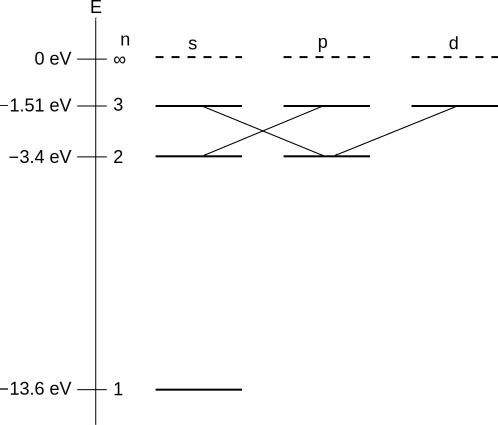
\includegraphics[width=100px]{figures/halphagrotrian.png}
\end{figure}
Both H\textsubscript{$\alpha$} and H\textsubscript{$\beta$} are in the visible spectrum, and so are easy to observe.

Other series are Lyman ($n_f=1$) and Paschen ($n_f=3$).
\end{frame}
\begin{frame}{\hydrogenspecrum}
Spectroscopy study of such emission can give information about the physical conditions in the plasma, such as density and temperature.

Advantage: No probes --- no interferance in any way with the plasma.

Disadvantage: Radiation is collected only along the lone of sight in the direction of observation.
\end{frame}
\begin{frame}{The emitted radiation process depends on:}
  The probability that 
 \begin{enumerate}
   \item there is an electron in the upper level of the transition,
   \item the electron transition is significant,
   \item the emitted photon escapes from the volume of the plasma without being absorbed.
 \end{enumerate} 
 We neglect process (3) and use the approximation of \emph{Optically thin plasma}.

 Values of the transition probabily $A_{i\to j}$ for process (2) are tabulated\footnote[frame]{See \url{https://physics.nist.gov/PhysRefData/ASD/lines_form.html} for example.}.
\end{frame}

\newcommand{\opticaldepth}{Optical Depth}
\begin{frame}{\opticaldepth}{Optically thin plasma}
  The optical depth $\tau$ (dimensionless) is a measure of the opacity of the element:
  \begin{equation*}
    \tau=-\kappa z
  \end{equation*}
  where $\kappa$ is the linear absorption coefficient (\si{\per\cm}).

  For a beam transferring through a plane medium (plasma in our case), $I_\text{out}$ and $I_\text{in}$ are related by
  \begin{equation*}
    I_\text{out} = I_\text{in}\mathrm{e}^{-\kappa z} %\tag{(Simplest)radiative transfer equation}
  \end{equation*}

\begin{figure}
    \centering
    \includegraphics[width=0.5\textwidth]{figures/radiativeTransfer.jpg}
\end{figure}

\end{frame}
\begin{frame}{\opticaldepth}{Optically thin plasma}
 \begin{center}
\begin{tabular}{ c c c }
  $\tau<1$ & $\longrightarrow$ & optically thin medium\\ 
  $\tau>1$ & $\longrightarrow$ & optically thick medium
\end{tabular}
\end{center}
By optically thin plasma we mean that the freely propagating radiation

is not significantly attenuated by the plasma environment, 

and reaches the detector without re--absorption.
\end{frame}
\newcommand{\lte}{Local Thermodynamic Equilibrium(LTE)}
\begin{frame}{\lte}
  In an isolated, closed system where the radiation and matter have reached equilibrium (black body cavity) the distribution of the kinetic motions, level populations and radiation fields are described by well-defined function of a single parameter ---

  The system temperature.

  This situation is called \emph{complete thermodynamic equilibrium}.
\end{frame}
\begin{frame}{\lte}
  \begin{center}
\resizebox{\textwidth}{!}{%
  \begin{tabular}{ c | c}
  Radiation field  & $\rho(\nu)=\frac{8\pi}{c^{3}}\frac{\nu^{3}}{\mathrm{e}^{\frac{h\nu}{k_{B}T}}-1}$ \\ \hline
  Ionisation degree  & $\frac{N_2}{N_1}=\frac{g_2}{g_1}\mathrm{e}^{-\frac{E_2-E_1}{k_BT}}$ \\ \hline %Eq 6.68 from Ryden and eq II.4 from Verdeyen
  Populations ratio of bound quantum states  & $f\left(v\right)=4\pi\left(\frac{m}{2\pi k_{B}T}\right)^{3/2}v^{2}\mathrm{e}^{-\frac{1}{2}\frac{mv^{2}}{k_{B}T}}$ % eq 2.2.4 from Moshe Elitzur.
  % Important : What is then equation 5.69 in Ryden??? See also Tallents 12.7
\end{tabular}
}
\end{center}
Each temperature would be different from each other, and become the same only for a system in thermodynamic equilibrium --- a black body cavity.

Those equilibrium populations are achieved because collisional process dominate the radiative processes.
\end{frame}
\begin{frame}{Collisional Processes}{And their inverses}
  \begin{center}
\resizebox{\textwidth}{!}{%
  \begin{tabular}{ c | c | c }
  Ionisation  & $ \left(\ \right)^{-1} \rightarrow$ & Recombination \\
  \hline
  Excitation  &  $\overset{\left(\:\right)^{-1}}{\longleftrightarrow}$ & De--excitation \\
  \hline
\end{tabular}
}
\end{center}
Inverse collisional processes have a \emph{detailed balance} relationship to each other.
% From Tallents, between equations 12.2 and 12.3:
In equilibrium, the principle of detailed balance requires these inverse processes to occur at equal rates.

\end{frame}
\begin{frame}{Detailed Balance Implications}
Thus, knowing the rate coefficient (cross section, for example) for one process, we can compute its inverse rate coefficient.

But those collisional--rate coefficients are simply atomic parameters\footnotemark, and so are independent of the state of the plasma, and apply also to plasmas not in equilibrium.


If no other process occur (apart from the detailed balance process) the populations have the equilibrium values for the particular density and temperature of the plasma.
\footnotetext{NIST.gov}
\end{frame}
\begin{frame}{Line Broadening}
A perfectly sharp energy line is impossible, and thus there is a distribution of transitions from states near $E_2$ to $E_1$.
\end{frame}
\section{Next Section}
\begin{frame}{text}
  Some dummy text.
\end{frame}
\end{document}